\subsection{Production and Mastering -- SDR On-Set and Digital Intermediate} \label{subsec:tv-onset-di-sdr}

\subsubsection{Summary}
It is common in the production of episodic television proudction to monitor the output of the camera on-set to check for framing, exposure, and often to create looks.  Looks are often created on-set or near-set using an on-set grading system with the result being a series of ASC-CDL values that are passed to digital intermediate (DI) mastering facility as a starting point for final grading.  In order to insure looks are set and communicated from on-set to the DI master facility as intended, it's important that the correct Output Transforms be used in each location.  The following is a recommendation for the usage of Output transforms for a common on-set to digital intermediate workflow.

\subsubsection{Workflow}
The complete workflow from camera to post is beyond the scope of this document, but Figure \ref{fig:workflow_tv-sdr-on-set-di} shows a typical workflow for the creation and communication of looks during episodic television production.

\begin{figure*}[ht!]
\centering
    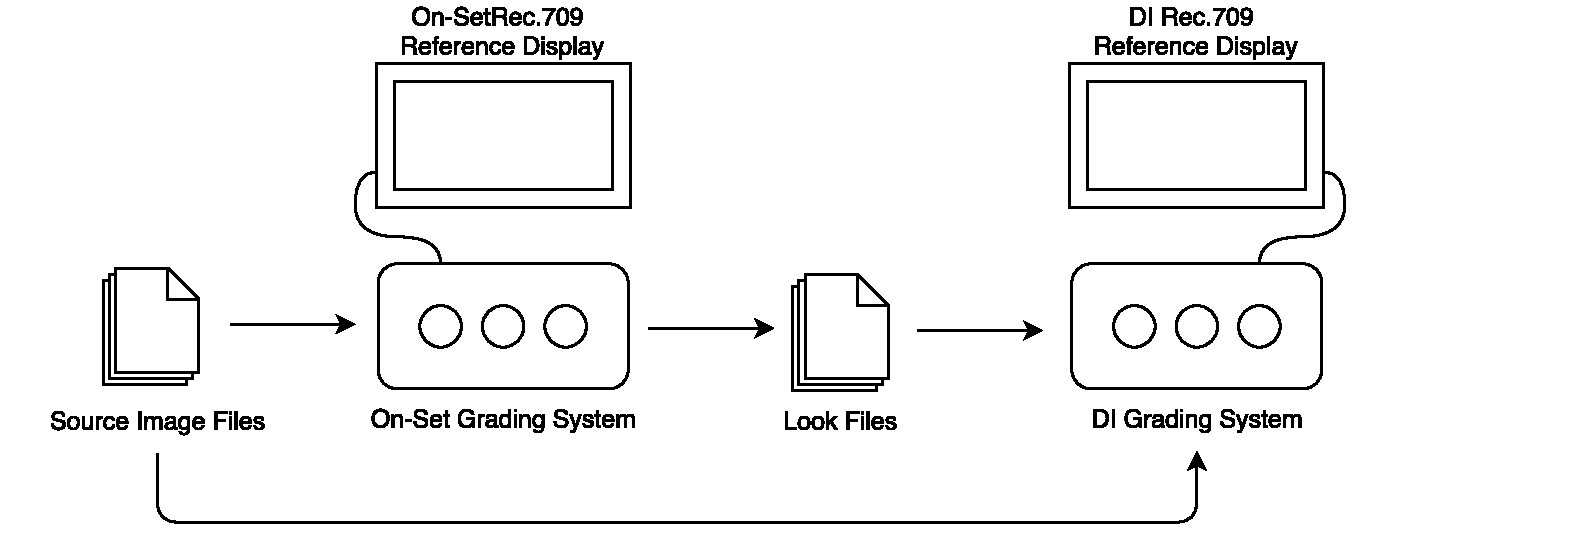
\includegraphics[width=4in]{images/workflows/workflow_tv-sdr-on-set-di.pdf}
    \caption{\small Episodic Television On-Set to SDR DI Workflow}
    \label{fig:workflow_tv-sdr-on-set-di}
\end{figure*}

In this on-set to digital intermediate workflow a Rec.709 reference display is connected to the on-set grading system and a high-end reference monitor is connected to the DI grading system.  In this workflow it is suggested that the on-set grading system be configured according to the Output Transform Application specified in section \ref{sec:odt-details-rec709}.  Likewise, the DI grading system should also be configured according to the output device transforms details specified in section \ref{sec:odt-details-rec709}.  The recommendations are summarized in Table \ref{tab:sum-tv-os-workflow}.

\begin{table}[ht!]
\centering
\begin{tabular}{|p{0.5in}|p{1.2in}|p{3.75in}|}
\hline
\textbf{System}   & \textbf{Display}            & \textbf{Suggested ODT}                                                  \\ \hline
On-set \newline Grading & Rec.709 Reference Monitor   & \texttt{\seqsplit{ODT.Academy.Rec709\_100nits\_dim.a1.0.3}} \\ \hline
DI \newline Grading & Rec.709 Reference Monitor & \texttt{\seqsplit{ODT.Academy.Rec709\_100nits\_dim.a1.0.3}}           \\ \hline
\end{tabular}
\caption[Workflows - Feature Film (Onset-DI) - Suggested ODTs]{Summary of suggested ODTs}
\label{tab:sum-ff-tv-workflow}
\end{table}
